\documentclass[a4paper,11pt]{article}

% ───────────────────────────
%         PACKAGES
% ───────────────────────────
\usepackage[utf8]{inputenc}
\usepackage[T1]{fontenc}
\usepackage{geometry}
\usepackage{graphicx}
\usepackage{amsmath, amssymb}
\usepackage{booktabs}
\usepackage{enumitem}
\usepackage{hyperref}
\usepackage{caption}
\usepackage{subcaption}

\usepackage{fancyhdr}
\usepackage{titlesec}
\usepackage{parskip}

\usepackage{minted}
\usepackage{inconsolata}  % clean monospaced font
\usepackage{mathpazo}     % professional text font

\usepackage{array}
\usepackage{booktabs}
\usepackage[table]{xcolor}


% ───────────────────────────
%         GEOMETRY
% ───────────────────────────
\geometry{
	a4paper,
	left=2.5cm,
	right=2.5cm,
	top=2.5cm,
	bottom=2.5cm
}

% ───────────────────────────
%         HEADER/FOOTER
% ───────────────────────────
\pagestyle{fancy}
\fancyhf{}
\renewcommand{\headrulewidth}{0.4pt}
\renewcommand{\footrulewidth}{0.4pt}
\lhead{\textsf{\textcolor{gray}{Python Notes}}}
\rhead{\textsf{\textcolor{gray}{Siddharth Patel}}}
\rfoot{\textsf{\textcolor{gray}{\thepage}}}

% ───────────────────────────
%         TITLE FORMAT
% ───────────────────────────
\titleformat{\section}
{\Large\bfseries\sffamily\color{black}}
{\thesection}{1em}{}

\titleformat{\subsection}
{\large\bfseries\sffamily\color{black}}
{\thesubsection}{1em}{}

% ───────────────────────────
%         MINTED SETTINGS
% ───────────────────────────
\definecolor{mintbg}{rgb}{0.97,0.97,0.97}
\setminted{
	bgcolor=mintbg,
	fontsize=\footnotesize,
	linenos=true,
	numbersep=5pt,
	frame=lines,
	framesep=2mm,
	breaklines=true,
	tabsize=4,
	encoding=utf8
}



% ───────────────────────────
%         TITLE PAGE
% ───────────────────────────
\title{\Huge \textbf{My Python Course Notes}\\[1ex]
	\Large Structured Revision for Every Lesson}
\author{\textbf{Siddharth Patel} \\ HTW Berlin}
\date{\today}

% ───────────────────────────
%         BEGIN DOCUMENT
% ───────────────────────────
\begin{document}
	
	\maketitle
	\thispagestyle{empty}
	\newpage
	\tableofcontents
	\newpage
	
	% ───────────────────────────
	%         FIRST LESSON
	% ───────────────────────────
	\section{Lesson 1: Print Function – Full Usage Guide}
	\inputminted{python}{Python_Files/print_guid.py}
	
	\vspace{1em}
	\subsection*{Additional Functions Used in This Lesson}
	
\vspace{1em}
\subsection*{Referenced Functions – Syntax and Output Type}

\rowcolors{2}{gray!10}{white}
\begin{tabular}{>{\bfseries}p{4cm} p{7.5cm} p{3cm}}
	\toprule
	Function & Syntax & Return / Output Type \\
	\midrule
	
	\texttt{with open()} & \texttt{with open("file.txt", "w") as f:} & File object \\
	\texttt{print(..., file=f)} & \texttt{print("text", file=f)} & Writes to file, returns \texttt{None} \\
	
	\texttt{range()} & \texttt{range(3)} or \texttt{range(start, stop, step)} & Range object (iterable) \\
	
	\texttt{time.sleep()} & \texttt{time.sleep(seconds)} & None (pauses execution) \\
	
	\bottomrule
\end{tabular}

	
	
	\section{Lesson 2: Input Function – Full Usage Guide}
	\inputminted{python}{Python_Files/input_guid.py}
	
	
	\vspace{1em}
	\subsection*{Referenced Functions – Syntax and Output Type}
	
	\rowcolors{2}{gray!10}{white}
	\begin{tabular}{>{\bfseries}p{3.5cm} p{8cm} p{3cm}}
		\toprule
		Function / Statement & Syntax & Return / Output Type \\
		\midrule
		
		\texttt{.split()} & \texttt{string.split()} or \texttt{string.split("delimiter")} & List of strings \\
		
		\texttt{map()} & \texttt{map(function, iterable)} & Map object (can be converted to list) \\
		
		\texttt{list()} & \texttt{list(iterable)} & List object \\
		
		\texttt{try / except} & 
		\texttt{try:\newline \hspace{1em} code\newline except ErrorType:\newline \hspace{1em} fallback} & Flow control – no return value; handles runtime errors \\
		
		\bottomrule
	\end{tabular}
	
	
	\section{Lesson 3: Math Operators – Full Usage Guide}
	\inputminted{python}{Python_Files/math_operators_guid.py}
	
	\section{Lesson 4: Strings – Full Usage Guide}
	\inputminted{python}{Python_Files/string_guid.py}
	
	\vspace{1em}
	\subsection*{Referenced Methods – Syntax and Output Type}
	
	\rowcolors{2}{gray!10}{white}
	\begin{tabular}{>{\bfseries}p{3.5cm} p{8cm} p{3cm}}
		\toprule
		Method / Function & Syntax & Return / Output Type \\
		\midrule
		
		\texttt{.capitalize()} & \texttt{str.capitalize()} & \texttt{str} \\
		
		\texttt{.lower()} & \texttt{str.lower()} & \texttt{str} \\
		
		\texttt{.title()} & \texttt{str.title()} & \texttt{str} \\
		
		\texttt{.casefold()} & \texttt{str.casefold()} & \texttt{str} \\
		
		\texttt{.upper()} & \texttt{str.upper()} & \texttt{str} \\
		
		\texttt{.count()} & \texttt{str.count(substring, start, end)} & \texttt{int} \\
		
		\texttt{.find()} & \texttt{str.find(substring, start, end)} & \texttt{int} \\
		
		\texttt{.replace()} & \texttt{str.replace(old, new, count)} & \texttt{str} \\
		
		\texttt{.swapcase()} & \texttt{str.swapcase()} & \texttt{str} \\
		
		\texttt{.join()} & \texttt{"separator".join(iterable)} & \texttt{str} \\
		
		\bottomrule
	\end{tabular}
	
	
	\section{Lesson 5: If, Else, and Conditional Operators}
	\inputminted{python}{Python_Files/if_else_guid.py}
	
	\vspace{1em}
	\subsection*{Referenced Operators – Syntax and Output Type}
	
	\rowcolors{2}{gray!10}{white}
	\begin{tabular}{>{\bfseries}p{4cm} p{7.5cm} p{3cm}}
		\toprule
		Operator & Syntax & Return / Output Type \\
		\midrule
		
		\texttt{==} (Equal) & \texttt{x == y} & \texttt{bool} \\
		
		\texttt{!=} (Not Equal) & \texttt{x != y} & \texttt{bool} \\
		
		\texttt{<} (Less Than) & \texttt{x < y} & \texttt{bool} \\
		
		\texttt{<=} (Less Than or Equal) & \texttt{x <= y} & \texttt{bool} \\
		
		\texttt{>} (Greater Than) & \texttt{x > y} & \texttt{bool} \\
		
		\texttt{>=} (Greater Than or Equal) & \texttt{x >= y} & \texttt{bool} \\
		
		\texttt{and} (Logical AND) & \texttt{x > 5 and x < 10} & \texttt{bool} \\
		
		\texttt{or} (Logical OR) & \texttt{x < 5 or x > 10} & \texttt{bool} \\
		
		\texttt{not} (Logical NOT) & \texttt{not (x > 5)} & \texttt{bool} \\
		
		\textit{Ternary Expression} & \texttt{value1 if condition else value2} & Result of \texttt{value1} or \texttt{value2} \\
		\bottomrule
	\end{tabular}
	
	\section{Lesson 6: While Loop – Full Usage Guide}
	\inputminted{python}{Python_Files/while_loop_guid.py}
	
	
	\vspace{1em}
	\subsection*{Referenced Keywords and Operators – Syntax and Output Type}
	
	\rowcolors{2}{gray!10}{white}
	\begin{tabular}{>{\bfseries}p{4cm} p{7.5cm} p{3cm}}
		\toprule
		Keyword / Operator & Syntax & Return / Effect \\
		\midrule
		
		\texttt{while} & \texttt{while condition:} & Repeats block while condition is \texttt{True} \\
		
		\texttt{break} & \texttt{break} & Immediately exits the nearest enclosing loop \\
		
		\texttt{continue} & \texttt{continue} & Skips current iteration and continues with the next \\
		
		\texttt{+=} & \texttt{x += y} & Updates: \texttt{x = x + y} \\
		
		\texttt{-=} & \texttt{x -= y} & Updates: \texttt{x = x - y} \\
		
		\texttt{*=} & \texttt{x *= y} & Updates: \texttt{x = x * y} \\
		
		\texttt{/=} & \texttt{x /= y} & Updates: \texttt{x = x / y} \\
		
		\texttt{++} / \texttt{--} & Not supported in Python & Causes \texttt{SyntaxError} \\
		
		\bottomrule
	\end{tabular}
	
	

	\section{Lesson 7: For Loop – Full Usage Guide}
	\inputminted{python}{Python_Files/for_loop_guid.py}
	
	\vspace{1em}
	\subsection*{Referenced Iteration Helpers – Syntax and Output Type}
	
	\rowcolors{2}{gray!10}{white}
	\begin{tabular}{>{\bfseries}p{4cm} p{7.5cm} p{3cm}}
		\toprule
		Function / Method & Syntax & Return / Output Type \\
		\midrule
		
		\texttt{tuple} & \texttt{(a, b, c)} & Iterable (ordered, immutable) \\
		
		\texttt{set} & \texttt{\{a, b, c\}} & Iterable (unordered, unique) \\
		
		\texttt{dict.items()} & \texttt{dict.items()} & Iterable of \texttt{(key, value)} pairs \\
		
		\texttt{enumerate()} & \texttt{enumerate(iterable)} & Iterable of \texttt{(index, item)} tuples \\
		
		\bottomrule
	\end{tabular}
	
	
	\section{Lesson 8: Functions – Full Usage Guide}
	\inputminted{python}{Python_Files/functions_guid.py}
	
	\section{Lesson 9: Lists – Introduction}
	\inputminted{python}{Python_Files/list_intro_guid.py}
	
	\vspace{1em}
	\subsection*{List Types and Creation Methods}
	
	\rowcolors{2}{gray!10}{white}
	\begin{tabular}{>{\bfseries}p{4.2cm} p{7cm} p{2.8cm}}
		\toprule
		List Type & Syntax / Example & Notes \\
		\midrule
		
		Homogeneous List & \texttt{[1, 2, 3, 4]} & All elements of the same type \\
		
		String List & \texttt{["apple", "banana"]} & List of strings \\
		
		Mixed-Type List & \texttt{["hi", 42, 3.14, True]} & Supports multiple data types \\
		
		Empty List & \texttt{[]} & No elements yet \\
		
		Nested List & \texttt{[[1, 2], [3, 4]]} & List inside a list \\
		
		From String & \texttt{list("abc")} & Converts string into list of characters \\
		
		From Range & \texttt{list(range(5))} & Converts range object into list \\
		
		\bottomrule
	\end{tabular}
	
	\section{Lesson 10: List Methods – General Usage}
	\inputminted{python}{Python_Files/list_methods_general.py}
	
	\vspace{1em}
	\subsection*{Common List Methods – Overview Table}
	
	\rowcolors{2}{gray!10}{white}
	\begin{tabular}{>{\bfseries}p{3.5cm} p{6cm} p{3.5cm}}
		\toprule
		Method & Description & Return Value \\
		\midrule
		
		\texttt{append(x)}   & Add element \texttt{x} to the end & \texttt{None} \\
		\texttt{insert(i,x)} & Insert \texttt{x} at index \texttt{i} & \texttt{None} \\
		\texttt{remove(x)}   & Remove first occurrence of \texttt{x} & \texttt{None} \\
		\texttt{pop(i)}      & Remove and return item at index \texttt{i} (last by default) & Element \\
		\texttt{clear()}     & Remove all items from the list & \texttt{None} \\
		\texttt{copy()}      & Return a shallow copy of the list & List copy \\
		\texttt{extend(iter)}& Append elements from iterable & \texttt{None} \\
		\texttt{index(x)}    & Return first index of \texttt{x} (error if not found) & Integer \\
		\texttt{count(x)}    & Count occurrences of \texttt{x} & Integer \\
		\texttt{reverse()}   & Reverse items in-place & \texttt{None} \\
		\texttt{sort()}      & Sort the list in-place & \texttt{None} \\
		
		\bottomrule
	\end{tabular}
	
	
	
	\section{Lesson 11: List Methods – Numeric Lists Only}
	\inputminted{python}{Python_Files/list_methods_numeric.py}
	
	\vspace{1em}
	\subsection*{List Methods for Numbers – Reference Table}
	
	\rowcolors{2}{gray!10}{white}
	\begin{tabular}{>{\bfseries}p{3.5cm} p{6cm} p{3.5cm}}
		\toprule
		Method & Description & Return Value \\
		\midrule
		
		\texttt{sort()}        & Sort list in ascending order (in-place) & \texttt{None} \\
		\texttt{reverse()}     & Reverse the list (in-place) & \texttt{None} \\
		\texttt{count(x)}      & Count how many times \texttt{x} appears & Integer \\
		\texttt{max(lst)}      & Return maximum element & Element \\
		\texttt{min(lst)}      & Return minimum element & Element \\
		\texttt{sum(lst)}      & Sum of all list items & Numeric \\
		\texttt{sorted(lst)}   & Return a new sorted list & New list \\
		\texttt{avg = sum()/len()} & Compute average (manual) & Float \\
		
		\bottomrule
	\end{tabular}
	
	
	\section{Lesson 12: 2D Lists and Nested Loops}
	\inputminted{python}{Python_Files/nested_list_guid.py}
	
	\section{Lesson 13: Tuples – Full Usage Guide}
	\inputminted{python}{Python_Files/tuples_guid.py}
	
	\vspace{1em}
	\subsection*{Tuple Functions – Syntax and Return Type}
	
	\rowcolors{2}{gray!10}{white}
	\begin{tabular}{>{\bfseries}p{3.5cm} p{7cm} p{3cm}}
		\toprule
		Function & Syntax & Return Type \\
		\midrule
		
		\texttt{len()} & \texttt{len(tuple)} & \texttt{int} (length of tuple) \\
		
		\texttt{max()} & \texttt{max(tuple)} & Largest item from tuple \\
		
		\texttt{min()} & \texttt{min(tuple)} & Smallest item from tuple \\
		
		\texttt{tuple()} & \texttt{tuple(iterable)} & A new tuple object \\
		
		\bottomrule
	\end{tabular}
	
	\section{Lesson 14: Sets – General Usage Guide}
	\inputminted{python}{Python_Files/sets_guid_general.py}
	
	\vspace{1em}
	\subsection*{General Set Methods – Syntax and Return Type}
	
	\rowcolors{2}{gray!10}{white}
	\begin{tabular}{>{\bfseries}p{3.5cm} p{7cm} p{3cm}}
		\toprule
		Method & Description & Return Type \\
		\midrule
		
		\texttt{add(x)}       & Adds element \texttt{x} to the set & \texttt{None} \\
		\texttt{remove(x)}    & Removes \texttt{x}; error if not found & \texttt{None} \\
		\texttt{discard(x)}   & Removes \texttt{x}; no error if not found & \texttt{None} \\
		\texttt{pop()}        & Removes and returns an arbitrary element & Element \\
		\texttt{clear()}      & Removes all items from the set & \texttt{None} \\
		\texttt{copy()}       & Returns a shallow copy of the set & Set copy \\
		\texttt{update(iter)} & Adds elements from another iterable & \texttt{None} \\
		
		\bottomrule
	\end{tabular}
	
	\section{Lesson 15: Sets – Mathematical Operations}
	\inputminted{python}{Python_Files/sets_math_guid.py}
	
	\vspace{1em}
	\subsection*{Set Operations – Syntax and Result}
	
	\rowcolors{2}{gray!10}{white}
	\begin{tabular}{>{\bfseries}p{4cm} p{6.5cm} p{3cm}}
		\toprule
		Method / Operator & Description & Return Type \\
		\midrule
		
		\texttt{a.union(b)} / \texttt{a | b} & All unique elements from both sets & New set \\
		\texttt{a.update(b)} & Adds all elements from b to a & \texttt{None} (in-place) \\
		
		\texttt{a.intersection(b)} / \texttt{a \& b} & Elements common to both sets & New set \\
		\texttt{a.intersection\_update(b)} & Keeps only common elements in a & \texttt{None} (in-place) \\
		
		\texttt{a.difference(b)} / \texttt{a - b} & Elements in a but not in b & New set \\
		\texttt{a.difference\_update(b)} & Removes items in b from a & \texttt{None} (in-place) \\
		
		\texttt{a.symmetric\_difference(b)} / \texttt{a \textasciicircum{} b} & Elements in a or b, not both & New set \\
		\texttt{a.symmetric\_difference\_update(b)} & Updates a to symmetric diff & \texttt{None} (in-place) \\
		
		\bottomrule
	\end{tabular}

\vspace{1em}
\subsection*{Set Comparison – Membership and Relationship}

\rowcolors{2}{gray!10}{white}
\begin{tabular}{>{\bfseries}p{4.5cm} p{7.2cm} p{2cm}}
	\toprule
	Method & Description & Returns \\
	\midrule
	
	\texttt{a.issubset(b)}     & True if all elements of a are in b     & Boolean \\
	\texttt{a.issuperset(b)}   & True if a contains all elements of b   & Boolean \\
	\texttt{a.isdisjoint(b)}   & True if a and b have no elements in common & Boolean \\
	
	\bottomrule
\end{tabular}

\vspace{1em}
\subsection*{Set Operations – Visual Explanation}

\renewcommand{\arraystretch}{1.8}
\rowcolors{2}{gray!10}{white}
\begin{tabular}{>{\bfseries}p{3.2cm} >{\centering\arraybackslash}p{3.5cm} p{6cm} >{\centering\arraybackslash}p{2.5cm}}
	\toprule
	Set Operation & Diagram & Explanation & \ttfamily In Python \\
	\midrule
	
	Union &
	\vspace{0.4em}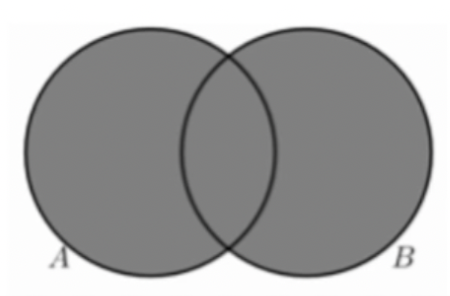
\includegraphics[width=2.8cm]{images/1.png} &
	$A \cup B$ is the set of all elements that are a member of $A$, or $B$, or both. &
	union() \\
	
	Intersection &
	\vspace{0.4em}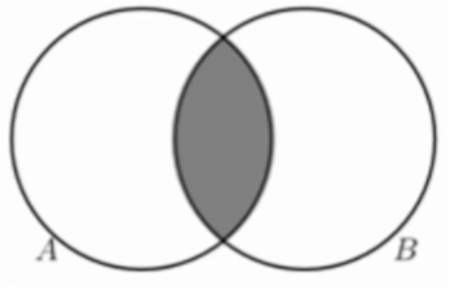
\includegraphics[width=2.8cm]{images/2.png} &
	$A \cap B$ is the set of all elements that are a member of both $A$ and $B$. &
	intersection() \\
	
	Difference &
	\vspace{0.4em}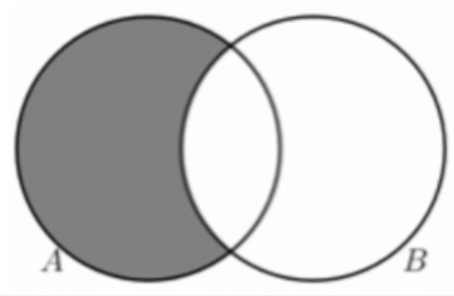
\includegraphics[width=2.8cm]{images/3.png} &
	$A \setminus B$ is the set of all elements of $A$ that are not in $B$. &
	difference() \\
	
	Symmetric Difference &
	\vspace{0.4em}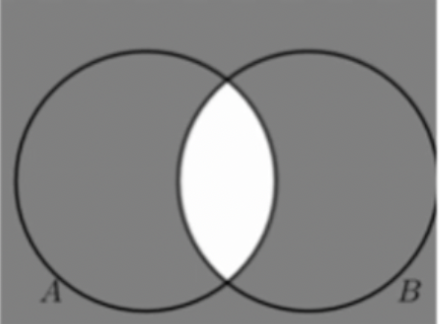
\includegraphics[width=2.8cm]{images/4.png} &
	$A \Delta B$ is the set of elements in either $A$ or $B$, but not both. &
	\shortstack{\\symmetric\\\_difference()} \\
	
	\bottomrule
\end{tabular}

\section{Lesson 16: Dictionary}
\inputminted{python}{Python_Files/dict_basics_guid.py}


\section{Lesson 17: Dictionary – Most Important Methods}
\inputminted{python}{Python_Files/dict_methods_guid.py}

\inputminted{python}{Python_Files/dict_key_value_item_get_examples.py}

\vspace{1em}
\subsection*{Common Dictionary Methods – Reference Table}

\rowcolors{2}{gray!10}{white}
\renewcommand{\arraystretch}{1.6}
\begin{tabular}{>{\bfseries}p{4cm} p{6.5cm} p{2.8cm}}
	\toprule
	Method & Description & Return Type \\
	\midrule
	
	\texttt{get(key, default)} & Returns value if key exists, else default or None & Value or None \\
	\texttt{keys()} & Returns all keys in the dictionary & dict\_keys view \\
	\texttt{values()} & Returns all values in the dictionary & dict\_values view \\
	\texttt{items()} & Returns key-value pairs as tuples & dict\_items view \\
	\texttt{pop(key)} & Removes and returns value for given key & Value \\
	\texttt{popitem()} & Removes and returns the last key-value pair & (key, value) tuple \\
	\texttt{update(dict)} & Updates dict with another dict or key-value pairs & None \\
	\texttt{clear()} & Removes all items from the dictionary & None \\
	\texttt{copy()} & Returns a shallow copy of the dictionary & New dict \\
	
	\bottomrule
\end{tabular}


	
	
	
\end{document}
